 \section{Parser Combinators for Path Querying}

Parser combinators provide a way to specify a language syntax in terms of functions and operations on them. 
A parser in this framework is usually a function which consumes a prefix of an input and returns either a parsing result or an error if the input is erroneous. 
Parsers can be composed by using a set of parser combinators to form more complex parsers. 
A parser combinators library provides with a set of basic combinators (such as sequential application or choice), and there can also be user-defined combinators. 
Most parser combinators libraries, including the Meerkat library, can only process the linear input --- strings or some kind of streams. 
We extend the Meerkat library to work on the graph input.


\subsection{Generic interface}

General input interface, as pointed in Trails
                             
\subsection{The set of combinators}

The basic combinators our library provides are presented in table~\ref{table:combinators}. 
Parsers for matching strings are implicitly generated whenever a string is used within a query. 
The classical same generation query~\cite{FndDB} can be written using the library as presented in Fig.~\ref{fig:query1Meerkat}.


\begin{table}[h]
\centering
\begin{tabular}{l@{}|l}
\multicolumn{1}{c|}{Combinator} & \multicolumn{1}{|c}{Description} \\ \hline
{\lstinline!a ~ b!} & sequential parsing: {\lstinline!a!} then {\lstinline!b!}   \\
{\lstinline!a | b!} & choice: {\lstinline!a!} or {\lstinline!b!}         \\
{\lstinline!a ?!}   & optional parsing: {\lstinline!a!} or nothing   \\
{\lstinline!a *!}   & repetition of zero or more {\lstinline!a!} \\
{\lstinline!a +!}   & repetition of at least one {\lstinline!a!} \\
{\lstinline!a ^ f!} & apply {\lstinline!f!} function to {\lstinline!a!} if  {\lstinline!a!} is a token \\
{\lstinline!a ^^!}  & capture output of {\lstinline!a!} if {\lstinline!a!} is a token    \\
{\lstinline!a & f!} & apply {\lstinline!f!} function to {\lstinline!a!} if  {\lstinline!a!} is a parser \\
{\lstinline!a &&!}  & capture output of {\lstinline!a!} if {\lstinline!a!} is a parser    \\
\end{tabular}
\caption{Meerkat combinators}
\label{table:combinators}
\end{table}


\begin{figure}[h]
\begin{lstlisting}
val S: Nonterminal = syn(
   "subclassof-1" ~ S.? ~ "subclassof" |
   "type-1" ~ S.? ~ "type")
\end{lstlisting}
\caption{The same generation query (Query 1) in Meerkat}
\label{fig:query1Meerkat}
\end{figure}


The most exciting feature of our library is that queries can be used as first-class values which means greater generalization and composition. 
The function \lstinline{sameGen} presented in Fig~\ref{fig:gen} is a generalization of the same generation query and is independent of the environment such as the input graph structure or other parsers.
It can be used for the creation of other queries, including the one presented in Fig~\ref{fig:query1Meerkat}: it is the result of the application of \lstinline{sameGen} to the appropriate relations (which can be treated as opening and closing brackets).
Another application of the \lstinline{sameGen} is a Query 2, which can be founded in Fig.~\ref{fig:query2Gen}.

\begin{figure}[h]
\begin{lstlisting}
val query1 = syn(sameGen(List(
    ("subclassof-1", "subclassof"),
    ("type-1", "type"))))
\end{lstlisting}
\caption{Query 1 as an application of \lstinline{sameGen}}
\label{fig:query1Gen}
\end{figure}

\begin{figure}[h]
\begin{lstlisting}

val g = new AnyRef {
      val P = syn(E((_: Int) > 0))
      val N = syn(E((_: Int) < 0))
      val S: Nonterminal[Int] = syn(P ~ N ~ S | P ~ N)
    }

 override def createParser: AbstractCPSParsers.AbstractSymbol[String, _, _] = {
    val num = V((_: String) forall Character.isDigit)
    syn(num ~ "+" ~ num)
  }

\end{lstlisting}
\caption{Example of predicates usage}
\label{fig:gen}
\end{figure}


\begin{figure}[h]
\begin{lstlisting}
def sameGen(brs) =
  bs.map { case (lbr, rbr) => 
             lbr ~ syn(sameGen(bs).?) ~ rbr } 
  match {
    case x :: Nil => syn(x)
    case x :: y :: xs => 
      syn(xs.foldLeft(x | y)(_ | _))
  }
\end{lstlisting}
\caption{Generic function for the same generations query}
\label{fig:gen}
\end{figure}

\subsection{An Example}
Let's assume we have a graph which consists of vertices of two types: movie vertex labeled with a movie's title and actor vertex labeled with actor's name. An actor can stars in a movie. This relation shown in graph as an edge with label $stars\_in$. Such graph is shown on \ref{fig:graph}. Let us capture one movie and one actor: Indiana Jones, and Harrison Ford, respectively. Now having that graph and two fixed vertices we would like to know all actors such they stars in Indiana Jones movie and also have at least another one common movie with Harrison Ford. In a terms of combinators we can define such query as the following: 

\begin{figure}[h]
\begin{lstlisting}
val actors  = syn(fixedActor ~ starsIn ~ fixedMovie ~ 
   hasActor ~ actor ~ starsIn ~ 
   movie ~ hasActor ~ fixedActor)
\end{lstlisting}
\caption{Actor combinator}
\label{fig:exampleQuery}
\end{figure}

Here \lstinline{actor} and \lstinline{movie} is a vertex combinator which parses a vertex which is a actor or movie which is not captured one, respectively. And \lstinline{fixedActor}, \lstinline{fixedMovie} combinators stands for captured one. Also,\lstinline{starsIn} and \lstinline{hasActor} are edge combinators which parses edges with corresponding label on them. Those combinator can be defined the following way:

\begin{figure}[h]
\begin{lstlisting}
val actor = syn(V(e => e.ntype == "actor" &&
  e.value() != "Harrison Ford"))
val movie = syn(V(e => e.ntype == "movie" && 
  e.value() != "Indiana Jones"))
val starsIn = syn(E(e => e.value() == "stars_in"))
val hasActor = syn(E(e => e.value() == "has_actor"))
val fixedActor = syn(V(e => e.ntype == "actor" &&
  e.value() == "Harrison Ford"))
val fixedMovie = syn(V(e => e.ntype == "movie" &&
  e.value() == "Indiana Jones"))
\end{lstlisting}
\caption{Combinators implementation}
\label{fig:combImpl}
\end{figure}

Now we would like, to get from our query only \lstinline{actor} combinator result. For that purpose let us modify it to make return result. In out library we have a \lstinline{^^} and \lstinline{&&} functions for that. Then we will have the following definition of our combinators:
\begin{figure}[h]
\begin{lstlisting}
val actor = syn(V(e => ...)^^)
val actors = syn((fixedActor ~ ... ~ fixedActor)&&)
\end{lstlisting}
\caption{Fixed combinators}
\label{fig:fixedAtor}
\end{figure}

Now we execute our query. For the graph presented on fig. \ref{fig:graph} we will get the only actor which satisfies given criteria Julian Glover.

A simplified SPPF for this query is presented in Fig.~\ref{fig:sppf}: rounded rectangles represent nonterminals and other rectangles represent productions. 
Every rectangle contains a nonterminal name or a production rule, as well as start and end nodes of the path in the input graph derived from the corresponding rectangle. 
Gray rectangles are start nonterminals.

\begin{figure}[h]
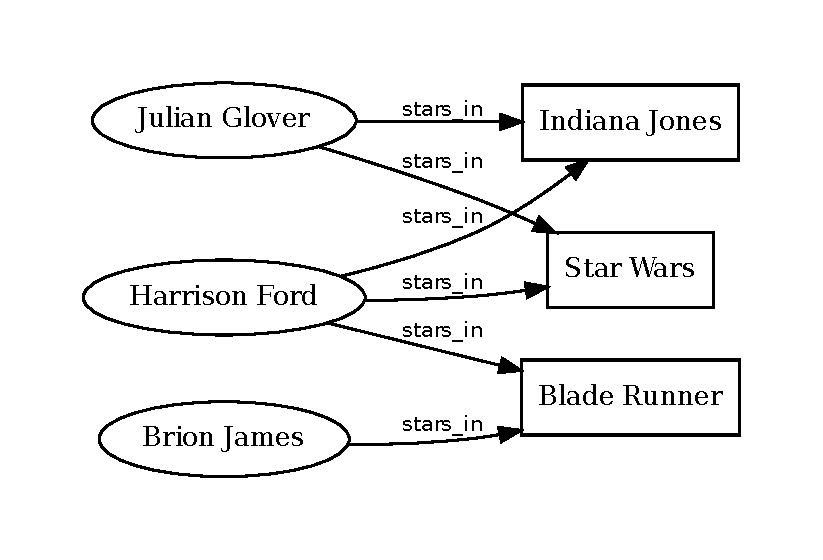
\includegraphics[width=0.45\textwidth]{graph}
% \begin{tikzpicture}[shorten >=1pt,node distance=3cm,on grid,auto] 
%    \node[state] (q_0)   {$0$}; 
%    \node[state] (q_1) [right=of q_0] {$1$}; 
%    \node[state] (q_2) [right=of q_1] {$2$}; 
%     \path[->] 
%     (q_0) edge[bend left, above]  node {$\text{subclassof}^{-1}$} (q_1)          
%     (q_1) edge[bend left, below]  node {$\text{subclassof}^{-1}$} (q_0)
%     (q_1) edge[bend left, above]  node {$\text{subclassof}$} (q_2)
%     (q_2) edge[bend left, below]  node {$\text{subclassof}$} (q_1);
% \end{tikzpicture}

\caption{Example Input graph}
\label{fig:graph}
\end{figure}

\begin{figure}[h]
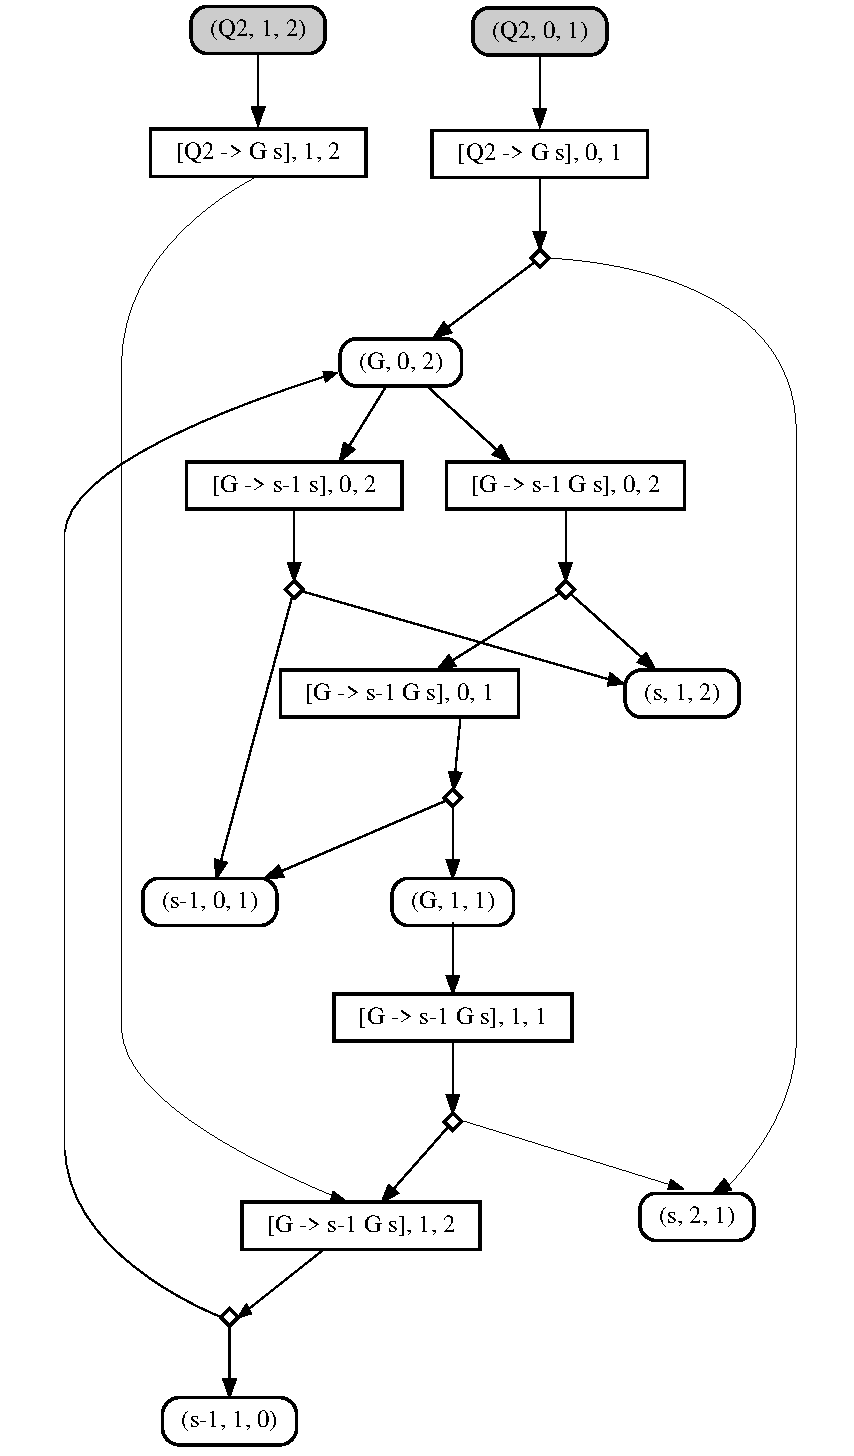
\includegraphics[scale=0.5]{sppf}
\caption{SPPF: result of applying actor/movie query to the graph~\ref{fig:graph}}
\label{fig:sppf}
\end{figure}
